\section{Experimental evaluation}
\label{sec:exp-eval}
\subsection{Dataset}
The dataset we used for experimental evaluation is VIRAT 2.0 \cite{virat20}. This dataset targets activity classification and is thus enriched with human activity, meaning all the frames mostly contain humans in motion. On the other hand, trespassing data is known to be extremely sparse. Therefore, we augment the VIRAT 2.0 dataset to control the amount of activity to background ratio as described below: 

\vspace{5pt}
\subsubsection{Synthetic dataset generator}
Figure \ref{fig:synthetic-dataset-generator} illustrates the black box model of our synthetic dataset generator. We adopt the following steps to generate the synthetic data: 
\begin{enumerate} 
    \item identify background frame
    \item make background block(s)
    \item write background block(s)
    \item write activity block(s)
    \item repeat (3) and (4)
\end{enumerate}

\begin{figure}
    \centering
    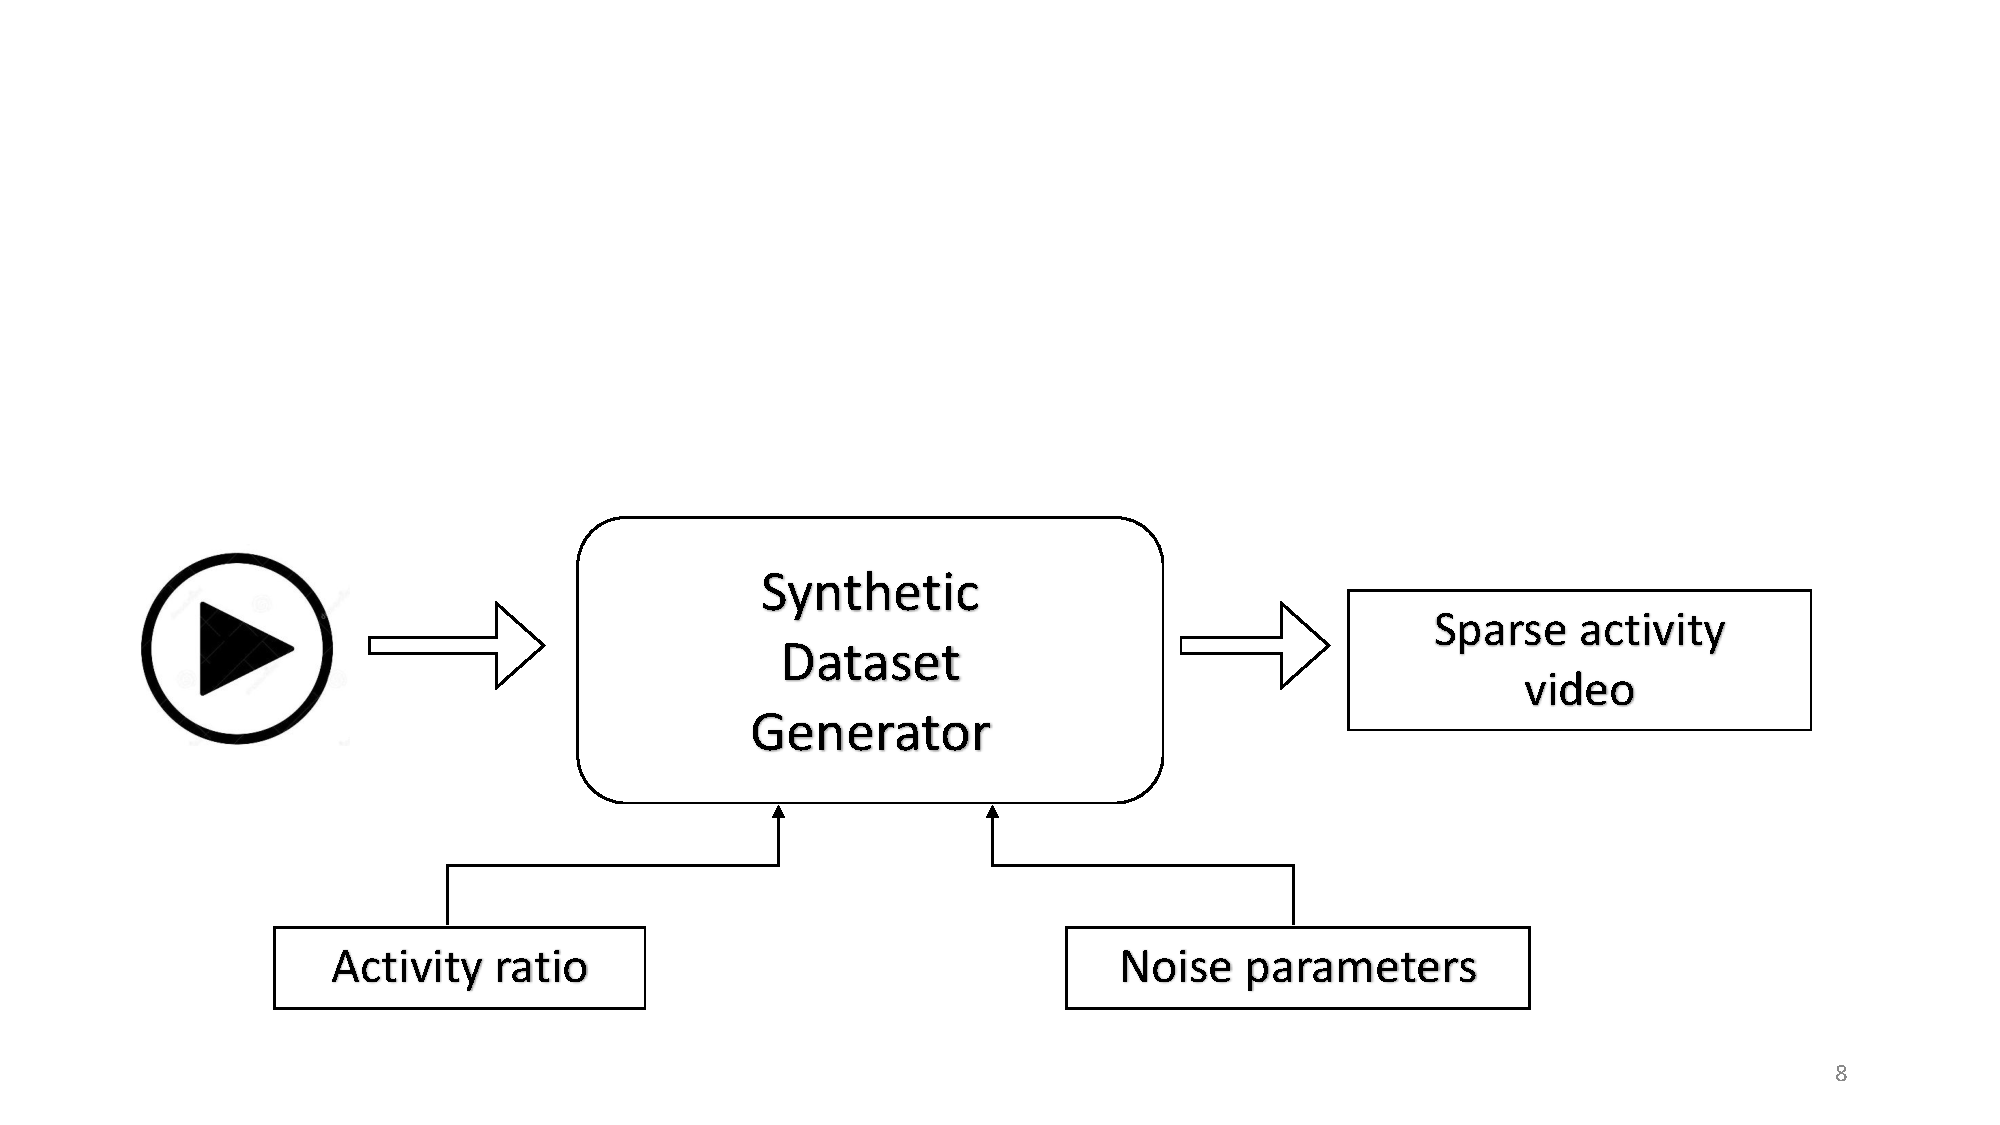
\includegraphics[width=\linewidth]{images/synthetic-dataset-generator}
    \caption{Synthetic dataset generator}
    \label{fig:synthetic-dataset-generator}
\end{figure}

Step 1 is human labor intensive but simple. We manually scroll through a video and identify a variety of frames with no human. We call these frames, the background frames. In step 2, we repeat each background frame $\Delta \times fps$ times to generate corresponding background block. Here, the $fps$ denotes the frames-per-second of the original video and $\Delta$ indicates the target length of background block in seconds. In step 3, we randomly select a certain number of  background blocks (determined in step 2) and write them to output video stream. Exact number of background blocks written depend on activity ratio, discussed at the end of this subsection. Step 4 writes the activity block in output video stream. An activity block is simply a section of the original video. By default, we use $30s$ long activity blocks. Length of each background block is also kept at $30s$ by default. Figure \ref{fig:synthetic-video} helps understand the concept of activity block and synthetic video.  

\begin{figure}
    \centering
    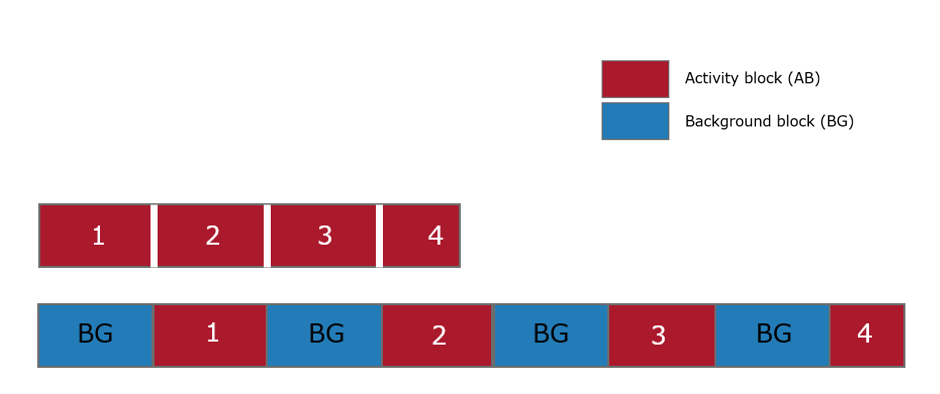
\includegraphics[width=\linewidth]{images/synthetic-video}
    \caption{Synthetic video illustration}
    \label{fig:synthetic-video}
\end{figure}

An important metric associated with this procedure is \textit{Activity Ratio}. It captures the fraction of activity present in the output synthetic video. It is defined as: 
$$ \text{Activity Ratio} = \text{AR} = \frac{1}{1+nBG} $$
where $nBG=$ number of background blocks per activity block. Figure \ref{fig:synthetic-video} has $nBG=1$. Table \ref{table:activity-ratio} explains the relationship between $nBG$ and AR. 


\begin{table}
\centering
\caption{Relationship of number of background blocks and activity ratio} \vspace{5pt}
\label{table:activity-ratio}
\begin{tabular}{@{}| l | l | l | @{}} \hline
nBG & nAB:nBG & AR   \\ \hline \hline
1   & 1:1     & 0.5  \\
3   & 1:3     & 0.25 \\
5   & 1:5     & 0.16 \\ \hline
\end{tabular}
\end{table}

\subsubsection{Adding noise}
Outdoor surveillance videos are often subjected to environmental challenges such as rain and snow. In order to test the robustness of our approach in those challenging situations, we add noise to our synthetic data. Salt and pepper noise \cite{marques2011practical} is known for modelling the rain and snow effect, therefore we use it in our experiments. 
Table \ref{table:noise-params} describes the parameters that control the level of noise. 

In order to add noise, we first select $p\%$ of frames from each background block. Each of the frames is equally likely to be selected. Now we draw an integer $r$ from the normal distribution with parameters $\mu$ and $\sigma$. For each selected frame, we select $r$ pixels and add noise to them. Again all pixels are equally likely. 

\begin{table}
\centering
\caption{Noise parameters}  \vspace{5pt}
\label{table:noise-params}
\begin{tabular}{|l|l|}
\hline
params & description                              \\ \hline \hline
$p$          & percentage of noisy frames in BG block  \\ 
$\mu$        & avg. number of noisy pixels in noisy frame     \\ 
$\sigma$     & standard deviation of number of noisy pixels     \\ \hline
\end{tabular}
\end{table}
